% Options for packages loaded elsewhere
\PassOptionsToPackage{unicode}{hyperref}
\PassOptionsToPackage{hyphens}{url}
%
\documentclass[
]{article}
\usepackage{lmodern}
\usepackage{amssymb,amsmath}
\usepackage{ifxetex,ifluatex}
\ifnum 0\ifxetex 1\fi\ifluatex 1\fi=0 % if pdftex
  \usepackage[T1]{fontenc}
  \usepackage[utf8]{inputenc}
  \usepackage{textcomp} % provide euro and other symbols
\else % if luatex or xetex
  \usepackage{unicode-math}
  \defaultfontfeatures{Scale=MatchLowercase}
  \defaultfontfeatures[\rmfamily]{Ligatures=TeX,Scale=1}
\fi
% Use upquote if available, for straight quotes in verbatim environments
\IfFileExists{upquote.sty}{\usepackage{upquote}}{}
\IfFileExists{microtype.sty}{% use microtype if available
  \usepackage[]{microtype}
  \UseMicrotypeSet[protrusion]{basicmath} % disable protrusion for tt fonts
}{}
\makeatletter
\@ifundefined{KOMAClassName}{% if non-KOMA class
  \IfFileExists{parskip.sty}{%
    \usepackage{parskip}
  }{% else
    \setlength{\parindent}{0pt}
    \setlength{\parskip}{6pt plus 2pt minus 1pt}}
}{% if KOMA class
  \KOMAoptions{parskip=half}}
\makeatother
\usepackage{xcolor}
\IfFileExists{xurl.sty}{\usepackage{xurl}}{} % add URL line breaks if available
\IfFileExists{bookmark.sty}{\usepackage{bookmark}}{\usepackage{hyperref}}
\hypersetup{
  pdftitle={CLASS\_06: R Functions},
  pdfauthor={Berenice R. Leal},
  hidelinks,
  pdfcreator={LaTeX via pandoc}}
\urlstyle{same} % disable monospaced font for URLs
\usepackage[margin=1in]{geometry}
\usepackage{color}
\usepackage{fancyvrb}
\newcommand{\VerbBar}{|}
\newcommand{\VERB}{\Verb[commandchars=\\\{\}]}
\DefineVerbatimEnvironment{Highlighting}{Verbatim}{commandchars=\\\{\}}
% Add ',fontsize=\small' for more characters per line
\usepackage{framed}
\definecolor{shadecolor}{RGB}{248,248,248}
\newenvironment{Shaded}{\begin{snugshade}}{\end{snugshade}}
\newcommand{\AlertTok}[1]{\textcolor[rgb]{0.94,0.16,0.16}{#1}}
\newcommand{\AnnotationTok}[1]{\textcolor[rgb]{0.56,0.35,0.01}{\textbf{\textit{#1}}}}
\newcommand{\AttributeTok}[1]{\textcolor[rgb]{0.77,0.63,0.00}{#1}}
\newcommand{\BaseNTok}[1]{\textcolor[rgb]{0.00,0.00,0.81}{#1}}
\newcommand{\BuiltInTok}[1]{#1}
\newcommand{\CharTok}[1]{\textcolor[rgb]{0.31,0.60,0.02}{#1}}
\newcommand{\CommentTok}[1]{\textcolor[rgb]{0.56,0.35,0.01}{\textit{#1}}}
\newcommand{\CommentVarTok}[1]{\textcolor[rgb]{0.56,0.35,0.01}{\textbf{\textit{#1}}}}
\newcommand{\ConstantTok}[1]{\textcolor[rgb]{0.00,0.00,0.00}{#1}}
\newcommand{\ControlFlowTok}[1]{\textcolor[rgb]{0.13,0.29,0.53}{\textbf{#1}}}
\newcommand{\DataTypeTok}[1]{\textcolor[rgb]{0.13,0.29,0.53}{#1}}
\newcommand{\DecValTok}[1]{\textcolor[rgb]{0.00,0.00,0.81}{#1}}
\newcommand{\DocumentationTok}[1]{\textcolor[rgb]{0.56,0.35,0.01}{\textbf{\textit{#1}}}}
\newcommand{\ErrorTok}[1]{\textcolor[rgb]{0.64,0.00,0.00}{\textbf{#1}}}
\newcommand{\ExtensionTok}[1]{#1}
\newcommand{\FloatTok}[1]{\textcolor[rgb]{0.00,0.00,0.81}{#1}}
\newcommand{\FunctionTok}[1]{\textcolor[rgb]{0.00,0.00,0.00}{#1}}
\newcommand{\ImportTok}[1]{#1}
\newcommand{\InformationTok}[1]{\textcolor[rgb]{0.56,0.35,0.01}{\textbf{\textit{#1}}}}
\newcommand{\KeywordTok}[1]{\textcolor[rgb]{0.13,0.29,0.53}{\textbf{#1}}}
\newcommand{\NormalTok}[1]{#1}
\newcommand{\OperatorTok}[1]{\textcolor[rgb]{0.81,0.36,0.00}{\textbf{#1}}}
\newcommand{\OtherTok}[1]{\textcolor[rgb]{0.56,0.35,0.01}{#1}}
\newcommand{\PreprocessorTok}[1]{\textcolor[rgb]{0.56,0.35,0.01}{\textit{#1}}}
\newcommand{\RegionMarkerTok}[1]{#1}
\newcommand{\SpecialCharTok}[1]{\textcolor[rgb]{0.00,0.00,0.00}{#1}}
\newcommand{\SpecialStringTok}[1]{\textcolor[rgb]{0.31,0.60,0.02}{#1}}
\newcommand{\StringTok}[1]{\textcolor[rgb]{0.31,0.60,0.02}{#1}}
\newcommand{\VariableTok}[1]{\textcolor[rgb]{0.00,0.00,0.00}{#1}}
\newcommand{\VerbatimStringTok}[1]{\textcolor[rgb]{0.31,0.60,0.02}{#1}}
\newcommand{\WarningTok}[1]{\textcolor[rgb]{0.56,0.35,0.01}{\textbf{\textit{#1}}}}
\usepackage{graphicx,grffile}
\makeatletter
\def\maxwidth{\ifdim\Gin@nat@width>\linewidth\linewidth\else\Gin@nat@width\fi}
\def\maxheight{\ifdim\Gin@nat@height>\textheight\textheight\else\Gin@nat@height\fi}
\makeatother
% Scale images if necessary, so that they will not overflow the page
% margins by default, and it is still possible to overwrite the defaults
% using explicit options in \includegraphics[width, height, ...]{}
\setkeys{Gin}{width=\maxwidth,height=\maxheight,keepaspectratio}
% Set default figure placement to htbp
\makeatletter
\def\fps@figure{htbp}
\makeatother
\setlength{\emergencystretch}{3em} % prevent overfull lines
\providecommand{\tightlist}{%
  \setlength{\itemsep}{0pt}\setlength{\parskip}{0pt}}
\setcounter{secnumdepth}{-\maxdimen} % remove section numbering

\title{CLASS\_06: R Functions}
\author{Berenice R. Leal}
\date{1/23/2020}

\begin{document}
\maketitle

\hypertarget{functions}{%
\section{Functions}\label{functions}}

\hypertarget{level-2-heding}{%
\subsection{Level 2 heding}\label{level-2-heding}}

\hypertarget{level-3-heading}{%
\subsubsection{Level 3 heading}\label{level-3-heading}}

\begin{Shaded}
\begin{Highlighting}[]
\CommentTok{# This is a silly plot}
\KeywordTok{plot}\NormalTok{(}\DecValTok{1}\OperatorTok{:}\DecValTok{5}\NormalTok{)}
\end{Highlighting}
\end{Shaded}

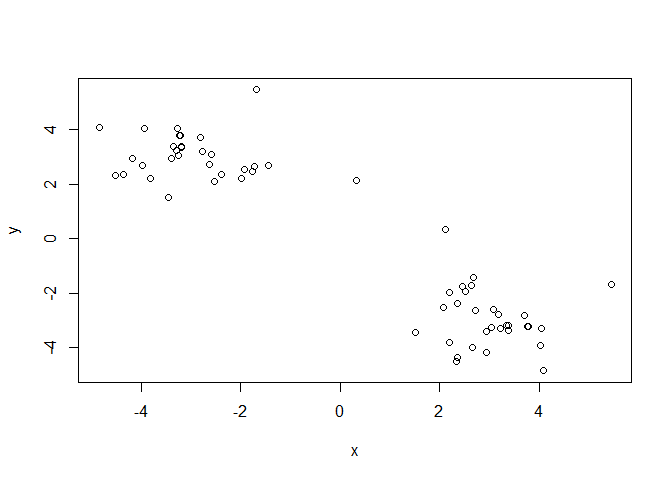
\includegraphics{CLASS_06_files/figure-latex/unnamed-chunk-1-1.pdf}

Lets see more about \textbf{file import} (i.e.~reading files into R). Th
main read function in base R is `read.table()'

\begin{Shaded}
\begin{Highlighting}[]
\KeywordTok{read.table}\NormalTok{(}\StringTok{"test1.txt"}\NormalTok{)}
\end{Highlighting}
\end{Shaded}

\begin{verbatim}
##               V1
## 1 Col1,Col2,Col3
## 2          1,2,3
## 3          4,5,6
## 4          7,8,9
## 5          a,b,c
\end{verbatim}

\begin{Shaded}
\begin{Highlighting}[]
\NormalTok{t1 <-}\StringTok{ }\KeywordTok{read.table}\NormalTok{(}\StringTok{"test1.txt"}\NormalTok{, }\DataTypeTok{sep=}\StringTok{","}\NormalTok{, }\DataTypeTok{header=}\OtherTok{TRUE}\NormalTok{)}
\NormalTok{t1}
\end{Highlighting}
\end{Shaded}

\begin{verbatim}
##   Col1 Col2 Col3
## 1    1    2    3
## 2    4    5    6
## 3    7    8    9
## 4    a    b    c
\end{verbatim}

Or I could just use `read.csv()' which has the arguents I want in this
case!

Second file

\begin{Shaded}
\begin{Highlighting}[]
\KeywordTok{read.table}\NormalTok{(}\StringTok{"test2.txt"}\NormalTok{, }\DataTypeTok{sep=}\StringTok{"$"}\NormalTok{, }\DataTypeTok{header=}\OtherTok{TRUE}\NormalTok{)}
\end{Highlighting}
\end{Shaded}

\begin{verbatim}
##   Col1 Col2 Col3
## 1    1    2    3
## 2    4    5    6
## 3    7    8    9
## 4    a    b    c
\end{verbatim}

\#Back to functions Our first example function

\begin{Shaded}
\begin{Highlighting}[]
\NormalTok{add <-}\StringTok{ }\ControlFlowTok{function}\NormalTok{ (x, }\DataTypeTok{y=}\DecValTok{1}\NormalTok{) \{ }
  \CommentTok{# Sum the inout x and y}
\NormalTok{  x }\OperatorTok{+}\StringTok{ }\NormalTok{y}
\NormalTok{\}}
\end{Highlighting}
\end{Shaded}

Let's try using this function

\begin{Shaded}
\begin{Highlighting}[]
\KeywordTok{add}\NormalTok{(}\DecValTok{7}\NormalTok{,}\DecValTok{3}\NormalTok{)}
\end{Highlighting}
\end{Shaded}

\begin{verbatim}
## [1] 10
\end{verbatim}

How does this work with vectors as input

\begin{Shaded}
\begin{Highlighting}[]
\KeywordTok{add}\NormalTok{( }\KeywordTok{c}\NormalTok{(}\DecValTok{1}\NormalTok{,}\DecValTok{2}\NormalTok{,}\DecValTok{4}\NormalTok{), }\DecValTok{4}\NormalTok{)}
\end{Highlighting}
\end{Shaded}

\begin{verbatim}
## [1] 5 6 8
\end{verbatim}

\begin{Shaded}
\begin{Highlighting}[]
\KeywordTok{add}\NormalTok{( }\KeywordTok{c}\NormalTok{(}\DecValTok{1}\NormalTok{,}\DecValTok{2}\NormalTok{,}\DecValTok{4}\NormalTok{), }\KeywordTok{c}\NormalTok{(}\DecValTok{1}\NormalTok{,}\DecValTok{2}\NormalTok{,}\DecValTok{4}\NormalTok{))}
\end{Highlighting}
\end{Shaded}

\begin{verbatim}
## [1] 2 4 8
\end{verbatim}

What is this `range()' function you talk of?

\begin{Shaded}
\begin{Highlighting}[]
\NormalTok{x <-}\StringTok{ }\KeywordTok{c}\NormalTok{(}\DecValTok{4}\NormalTok{,}\DecValTok{4}\NormalTok{,}\DecValTok{10}\NormalTok{,}\DecValTok{3}\NormalTok{,}\DecValTok{11}\NormalTok{)}
\KeywordTok{max}\NormalTok{(x)}
\end{Highlighting}
\end{Shaded}

\begin{verbatim}
## [1] 11
\end{verbatim}

\begin{Shaded}
\begin{Highlighting}[]
\KeywordTok{min}\NormalTok{(x)}
\end{Highlighting}
\end{Shaded}

\begin{verbatim}
## [1] 3
\end{verbatim}

\begin{Shaded}
\begin{Highlighting}[]
\KeywordTok{range}\NormalTok{(x)}
\end{Highlighting}
\end{Shaded}

\begin{verbatim}
## [1]  3 11
\end{verbatim}

This is our second function:

\begin{Shaded}
\begin{Highlighting}[]
\NormalTok{rescale <-}\StringTok{ }\ControlFlowTok{function}\NormalTok{(x) \{}
\NormalTok{ rng <-}\StringTok{ }\KeywordTok{range}\NormalTok{(x)}
\NormalTok{ (x }\OperatorTok{-}\StringTok{ }\NormalTok{rng[}\DecValTok{1}\NormalTok{]) }\OperatorTok{/}\StringTok{ }\NormalTok{(rng[}\DecValTok{2}\NormalTok{] }\OperatorTok{-}\StringTok{ }\NormalTok{rng[}\DecValTok{1}\NormalTok{])}
\NormalTok{\}}

\KeywordTok{rescale}\NormalTok{(x)}
\end{Highlighting}
\end{Shaded}

\begin{verbatim}
## [1] 0.125 0.125 0.875 0.000 1.000
\end{verbatim}

\begin{Shaded}
\begin{Highlighting}[]
\KeywordTok{rescale}\NormalTok{ (}\DecValTok{1}\OperatorTok{:}\DecValTok{10}\NormalTok{)}
\end{Highlighting}
\end{Shaded}

\begin{verbatim}
##  [1] 0.0000000 0.1111111 0.2222222 0.3333333 0.4444444 0.5555556 0.6666667
##  [8] 0.7777778 0.8888889 1.0000000
\end{verbatim}

\begin{Shaded}
\begin{Highlighting}[]
\CommentTok{#How would you get your function to work here...}
\KeywordTok{rescale}\NormalTok{( }\KeywordTok{c}\NormalTok{(}\DecValTok{1}\NormalTok{,}\DecValTok{2}\NormalTok{,}\OtherTok{NA}\NormalTok{,}\DecValTok{3}\NormalTok{,}\DecValTok{10}\NormalTok{))}
\end{Highlighting}
\end{Shaded}

\begin{verbatim}
## [1] NA NA NA NA NA
\end{verbatim}

\begin{Shaded}
\begin{Highlighting}[]
\NormalTok{x <-}\StringTok{ }\KeywordTok{c}\NormalTok{(}\DecValTok{1}\NormalTok{,}\DecValTok{2}\NormalTok{, }\OtherTok{NA}\NormalTok{, }\DecValTok{3}\NormalTok{,}\DecValTok{10}\NormalTok{)}
\NormalTok{rng <-}\StringTok{ }\KeywordTok{range}\NormalTok{(x)}
\NormalTok{rng}
\end{Highlighting}
\end{Shaded}

\begin{verbatim}
## [1] NA NA
\end{verbatim}

\begin{Shaded}
\begin{Highlighting}[]
\NormalTok{rng <-}\StringTok{ }\KeywordTok{range}\NormalTok{(x, }\DataTypeTok{na.rm =} \OtherTok{TRUE}\NormalTok{)}
\NormalTok{rng}
\end{Highlighting}
\end{Shaded}

\begin{verbatim}
## [1]  1 10
\end{verbatim}

\begin{Shaded}
\begin{Highlighting}[]
\NormalTok{rescale2 <-}\StringTok{ }\ControlFlowTok{function}\NormalTok{(x) \{}
\NormalTok{ rng <-}\StringTok{ }\KeywordTok{range}\NormalTok{(x, }\DataTypeTok{na.rm=}\OtherTok{TRUE}\NormalTok{)}
\NormalTok{ (x }\OperatorTok{-}\StringTok{ }\NormalTok{rng[}\DecValTok{1}\NormalTok{]) }\OperatorTok{/}\StringTok{ }\NormalTok{(rng[}\DecValTok{2}\NormalTok{] }\OperatorTok{-}\StringTok{ }\NormalTok{rng[}\DecValTok{1}\NormalTok{])}
\NormalTok{\}}
\end{Highlighting}
\end{Shaded}

\begin{Shaded}
\begin{Highlighting}[]
\KeywordTok{rescale2}\NormalTok{( }\KeywordTok{c}\NormalTok{(}\DecValTok{1}\NormalTok{,}\DecValTok{2}\NormalTok{,}\OtherTok{NA}\NormalTok{,}\DecValTok{3}\NormalTok{,}\DecValTok{10}\NormalTok{) )}
\end{Highlighting}
\end{Shaded}

\begin{verbatim}
## [1] 0.0000000 0.1111111        NA 0.2222222 1.0000000
\end{verbatim}

\begin{Shaded}
\begin{Highlighting}[]
\NormalTok{rescale3 <-}\StringTok{ }\ControlFlowTok{function}\NormalTok{(x, }\DataTypeTok{na.rm=}\OtherTok{TRUE}\NormalTok{, }\DataTypeTok{plot=}\OtherTok{FALSE}\NormalTok{) \{}
\NormalTok{ rng <-}\KeywordTok{range}\NormalTok{(x, }\DataTypeTok{na.rm=}\NormalTok{na.rm)}
 \KeywordTok{print}\NormalTok{(}\StringTok{"Hello"}\NormalTok{)}
 
\NormalTok{ answer <-}\StringTok{ }\NormalTok{(x }\OperatorTok{-}\StringTok{ }\NormalTok{rng[}\DecValTok{1}\NormalTok{]) }\OperatorTok{/}\StringTok{ }\NormalTok{(rng[}\DecValTok{2}\NormalTok{] }\OperatorTok{-}\StringTok{ }\NormalTok{rng[}\DecValTok{1}\NormalTok{])}
 
 \KeywordTok{print}\NormalTok{(}\StringTok{"dont sing again"}\NormalTok{)}
 
 \ControlFlowTok{if}\NormalTok{(plot) \{}
 \KeywordTok{plot}\NormalTok{(answer, }\DataTypeTok{typ=}\StringTok{"b"}\NormalTok{, }\DataTypeTok{lwd=}\DecValTok{4}\NormalTok{)}
\NormalTok{ \}}
 \KeywordTok{print}\NormalTok{(}\StringTok{"I can see it in ..."}\NormalTok{)}
 \KeywordTok{return}\NormalTok{(answer)}
\NormalTok{\}}
\end{Highlighting}
\end{Shaded}

\begin{Shaded}
\begin{Highlighting}[]
\KeywordTok{rescale3}\NormalTok{(x, }\DataTypeTok{plot=}\OtherTok{TRUE}\NormalTok{)}
\end{Highlighting}
\end{Shaded}

\begin{verbatim}
## [1] "Hello"
## [1] "dont sing again"
\end{verbatim}

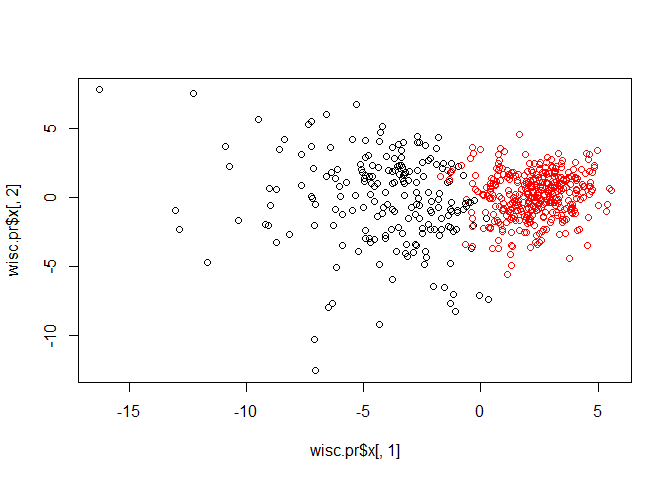
\includegraphics{CLASS_06_files/figure-latex/unnamed-chunk-17-1.pdf}

\begin{verbatim}
## [1] "I can see it in ..."
\end{verbatim}

\begin{verbatim}
## [1] 0.0000000 0.1111111        NA 0.2222222 1.0000000
\end{verbatim}

PART B

Hands on Section

\begin{Shaded}
\begin{Highlighting}[]
\KeywordTok{library}\NormalTok{(bio3d)}
\NormalTok{s1 <-}\StringTok{ }\KeywordTok{read.pdb}\NormalTok{(}\StringTok{"4AKE"}\NormalTok{) }\CommentTok{# kinase with drug}
\end{Highlighting}
\end{Shaded}

\begin{verbatim}
##   Note: Accessing on-line PDB file
\end{verbatim}

\begin{Shaded}
\begin{Highlighting}[]
\NormalTok{s2 <-}\StringTok{ }\KeywordTok{read.pdb}\NormalTok{(}\StringTok{"1AKE"}\NormalTok{) }\CommentTok{# kinase no drug}
\end{Highlighting}
\end{Shaded}

\begin{verbatim}
##   Note: Accessing on-line PDB file
##    PDB has ALT records, taking A only, rm.alt=TRUE
\end{verbatim}

\begin{Shaded}
\begin{Highlighting}[]
\NormalTok{s3 <-}\StringTok{ }\KeywordTok{read.pdb}\NormalTok{(}\StringTok{"1E4Y"}\NormalTok{) }\CommentTok{# kinase with drug}
\end{Highlighting}
\end{Shaded}

\begin{verbatim}
##   Note: Accessing on-line PDB file
\end{verbatim}

\begin{Shaded}
\begin{Highlighting}[]
\NormalTok{s1.chainA <-}\StringTok{ }\KeywordTok{trim.pdb}\NormalTok{(s1, }\DataTypeTok{chain=}\StringTok{"A"}\NormalTok{, }\DataTypeTok{elety=}\StringTok{"CA"}\NormalTok{)}
\NormalTok{s2.chainA <-}\StringTok{ }\KeywordTok{trim.pdb}\NormalTok{(s2, }\DataTypeTok{chain=}\StringTok{"A"}\NormalTok{, }\DataTypeTok{elety=}\StringTok{"CA"}\NormalTok{)}
\NormalTok{s3.chainA <-}\StringTok{ }\KeywordTok{trim.pdb}\NormalTok{(s3, }\DataTypeTok{chain=}\StringTok{"A"}\NormalTok{, }\DataTypeTok{elety=}\StringTok{"CA"}\NormalTok{)}

\NormalTok{s1.b <-}\StringTok{ }\NormalTok{s1.chainA}\OperatorTok{$}\NormalTok{atom}\OperatorTok{$}\NormalTok{b}
\NormalTok{s2.b <-}\StringTok{ }\NormalTok{s2.chainA}\OperatorTok{$}\NormalTok{atom}\OperatorTok{$}\NormalTok{b}
\NormalTok{s3.b <-}\StringTok{ }\NormalTok{s3.chainA}\OperatorTok{$}\NormalTok{atom}\OperatorTok{$}\NormalTok{b}

\KeywordTok{plotb3}\NormalTok{(s1.b, }\DataTypeTok{sse=}\NormalTok{s1.chainA, }\DataTypeTok{typ=}\StringTok{"l"}\NormalTok{, }\DataTypeTok{ylab=}\StringTok{"Bfactor"}\NormalTok{)}
\end{Highlighting}
\end{Shaded}

\includegraphics{CLASS_06_files/figure-latex/unnamed-chunk-18-1.pdf}

\begin{Shaded}
\begin{Highlighting}[]
\KeywordTok{plotb3}\NormalTok{(s2.b, }\DataTypeTok{sse=}\NormalTok{s2.chainA, }\DataTypeTok{typ=}\StringTok{"l"}\NormalTok{, }\DataTypeTok{ylab=}\StringTok{"Bfactor"}\NormalTok{)}
\end{Highlighting}
\end{Shaded}

\includegraphics{CLASS_06_files/figure-latex/unnamed-chunk-18-2.pdf}

\begin{Shaded}
\begin{Highlighting}[]
\KeywordTok{plotb3}\NormalTok{(s3.b, }\DataTypeTok{sse=}\NormalTok{s3.chainA, }\DataTypeTok{typ=}\StringTok{"l"}\NormalTok{, }\DataTypeTok{ylab=}\StringTok{"Bfactor"}\NormalTok{)}
\end{Highlighting}
\end{Shaded}

\includegraphics{CLASS_06_files/figure-latex/unnamed-chunk-18-3.pdf}

\begin{Shaded}
\begin{Highlighting}[]
\NormalTok{s1 <-}\StringTok{ }\KeywordTok{read.pdb}\NormalTok{(}\StringTok{"4AKE"}\NormalTok{) }\CommentTok{# kinase with drug}
\end{Highlighting}
\end{Shaded}

\begin{verbatim}
##   Note: Accessing on-line PDB file
\end{verbatim}

\begin{verbatim}
## Warning in get.pdb(file, path = tempdir(), verbose = FALSE): C:
## \Users\Admin\AppData\Local\Temp\RtmpgxgdfH/4AKE.pdb exists. Skipping download
\end{verbatim}

\begin{Shaded}
\begin{Highlighting}[]
\NormalTok{s1}
\end{Highlighting}
\end{Shaded}

\begin{verbatim}
## 
##  Call:  read.pdb(file = "4AKE")
## 
##    Total Models#: 1
##      Total Atoms#: 3459,  XYZs#: 10377  Chains#: 2  (values: A B)
## 
##      Protein Atoms#: 3312  (residues/Calpha atoms#: 428)
##      Nucleic acid Atoms#: 0  (residues/phosphate atoms#: 0)
## 
##      Non-protein/nucleic Atoms#: 147  (residues: 147)
##      Non-protein/nucleic resid values: [ HOH (147) ]
## 
##    Protein sequence:
##       MRIILLGAPGAGKGTQAQFIMEKYGIPQISTGDMLRAAVKSGSELGKQAKDIMDAGKLVT
##       DELVIALVKERIAQEDCRNGFLLDGFPRTIPQADAMKEAGINVDYVLEFDVPDELIVDRI
##       VGRRVHAPSGRVYHVKFNPPKVEGKDDVTGEELTTRKDDQEETVRKRLVEYHQMTAPLIG
##       YYSKEAEAGNTKYAKVDGTKPVAEVRADLEKILGMRIILLGAPGA...<cut>...KILG
## 
## + attr: atom, xyz, seqres, helix, sheet,
##         calpha, remark, call
\end{verbatim}

Q1. What type of object is returned from the `read.pdb()' It is a list
of 8 things and of class

\begin{Shaded}
\begin{Highlighting}[]
\KeywordTok{class}\NormalTok{(s1)}
\end{Highlighting}
\end{Shaded}

\begin{verbatim}
## [1] "pdb" "sse"
\end{verbatim}

\begin{Shaded}
\begin{Highlighting}[]
\KeywordTok{str}\NormalTok{(s1)}
\end{Highlighting}
\end{Shaded}

\begin{verbatim}
## List of 8
##  $ atom  :'data.frame':  3459 obs. of  16 variables:
##   ..$ type  : chr [1:3459] "ATOM" "ATOM" "ATOM" "ATOM" ...
##   ..$ eleno : int [1:3459] 1 2 3 4 5 6 7 8 9 10 ...
##   ..$ elety : chr [1:3459] "N" "CA" "C" "O" ...
##   ..$ alt   : chr [1:3459] NA NA NA NA ...
##   ..$ resid : chr [1:3459] "MET" "MET" "MET" "MET" ...
##   ..$ chain : chr [1:3459] "A" "A" "A" "A" ...
##   ..$ resno : int [1:3459] 1 1 1 1 1 1 1 1 2 2 ...
##   ..$ insert: chr [1:3459] NA NA NA NA ...
##   ..$ x     : num [1:3459] -10.93 -9.9 -9.17 -9.8 -10.59 ...
##   ..$ y     : num [1:3459] -24.9 -24.4 -23.3 -22.3 -24 ...
##   ..$ z     : num [1:3459] -9.52 -10.48 -9.81 -9.35 -11.77 ...
##   ..$ o     : num [1:3459] 1 1 1 1 1 1 1 1 1 1 ...
##   ..$ b     : num [1:3459] 41.5 29 27.9 26.4 34.2 ...
##   ..$ segid : chr [1:3459] NA NA NA NA ...
##   ..$ elesy : chr [1:3459] "N" "C" "C" "O" ...
##   ..$ charge: chr [1:3459] NA NA NA NA ...
##  $ xyz   : 'xyz' num [1, 1:10377] -10.93 -24.89 -9.52 -9.9 -24.42 ...
##  $ seqres: Named chr [1:428] "MET" "ARG" "ILE" "ILE" ...
##   ..- attr(*, "names")= chr [1:428] "A" "A" "A" "A" ...
##  $ helix :List of 4
##   ..$ start: Named num [1:19] 13 31 44 61 75 90 113 161 202 13 ...
##   .. ..- attr(*, "names")= chr [1:19] "" "" "" "" ...
##   ..$ end  : Named num [1:19] 24 40 54 73 77 98 121 187 213 24 ...
##   .. ..- attr(*, "names")= chr [1:19] "" "" "" "" ...
##   ..$ chain: chr [1:19] "A" "A" "A" "A" ...
##   ..$ type : chr [1:19] "5" "1" "1" "1" ...
##  $ sheet :List of 4
##   ..$ start: Named num [1:14] 192 105 2 81 27 123 131 192 105 2 ...
##   .. ..- attr(*, "names")= chr [1:14] "" "" "" "" ...
##   ..$ end  : Named num [1:14] 197 110 7 84 29 126 134 197 110 7 ...
##   .. ..- attr(*, "names")= chr [1:14] "" "" "" "" ...
##   ..$ chain: chr [1:14] "A" "A" "A" "A" ...
##   ..$ sense: chr [1:14] "0" "1" "1" "1" ...
##  $ calpha: logi [1:3459] FALSE TRUE FALSE FALSE FALSE FALSE ...
##  $ remark:List of 1
##   ..$ biomat:List of 4
##   .. ..$ num   : int 1
##   .. ..$ chain :List of 1
##   .. .. ..$ : chr [1:2] "A" "B"
##   .. ..$ mat   :List of 1
##   .. .. ..$ :List of 1
##   .. .. .. ..$ A B: num [1:3, 1:4] 1 0 0 0 1 0 0 0 1 0 ...
##   .. ..$ method: chr "AUTHOR"
##  $ call  : language read.pdb(file = "4AKE")
##  - attr(*, "class")= chr [1:2] "pdb" "sse"
\end{verbatim}

Q2. What does the trim.pdb() function do?

\begin{Shaded}
\begin{Highlighting}[]
\NormalTok{s1.chainA <-}\StringTok{ }\KeywordTok{trim.pdb}\NormalTok{(s1, }\DataTypeTok{chain=}\StringTok{"A"}\NormalTok{, }\DataTypeTok{elety=}\StringTok{"CA"}\NormalTok{)}
\NormalTok{s1}
\end{Highlighting}
\end{Shaded}

\begin{verbatim}
## 
##  Call:  read.pdb(file = "4AKE")
## 
##    Total Models#: 1
##      Total Atoms#: 3459,  XYZs#: 10377  Chains#: 2  (values: A B)
## 
##      Protein Atoms#: 3312  (residues/Calpha atoms#: 428)
##      Nucleic acid Atoms#: 0  (residues/phosphate atoms#: 0)
## 
##      Non-protein/nucleic Atoms#: 147  (residues: 147)
##      Non-protein/nucleic resid values: [ HOH (147) ]
## 
##    Protein sequence:
##       MRIILLGAPGAGKGTQAQFIMEKYGIPQISTGDMLRAAVKSGSELGKQAKDIMDAGKLVT
##       DELVIALVKERIAQEDCRNGFLLDGFPRTIPQADAMKEAGINVDYVLEFDVPDELIVDRI
##       VGRRVHAPSGRVYHVKFNPPKVEGKDDVTGEELTTRKDDQEETVRKRLVEYHQMTAPLIG
##       YYSKEAEAGNTKYAKVDGTKPVAEVRADLEKILGMRIILLGAPGA...<cut>...KILG
## 
## + attr: atom, xyz, seqres, helix, sheet,
##         calpha, remark, call
\end{verbatim}

Q4. What would be a better plot to compare across the different
proteins? 1 plot with all the graphs in it

\begin{Shaded}
\begin{Highlighting}[]
\KeywordTok{plotb3}\NormalTok{(s1.b, }\DataTypeTok{sse=}\NormalTok{s1.chainA, }\DataTypeTok{typ=}\StringTok{"l"}\NormalTok{, }\DataTypeTok{ylab=}\StringTok{"Bfactor"}\NormalTok{)}
\KeywordTok{points}\NormalTok{(s2.b, }\DataTypeTok{typ=}\StringTok{"l"}\NormalTok{, }\DataTypeTok{col=}\StringTok{"blue"}\NormalTok{, }\DataTypeTok{lwd=}\DecValTok{2}\NormalTok{)}
\KeywordTok{points}\NormalTok{(s3.b, }\DataTypeTok{typ=}\StringTok{"l"}\NormalTok{, }\DataTypeTok{col=}\StringTok{"red"}\NormalTok{, }\DataTypeTok{lwd=}\DecValTok{2}\NormalTok{)}
\end{Highlighting}
\end{Shaded}

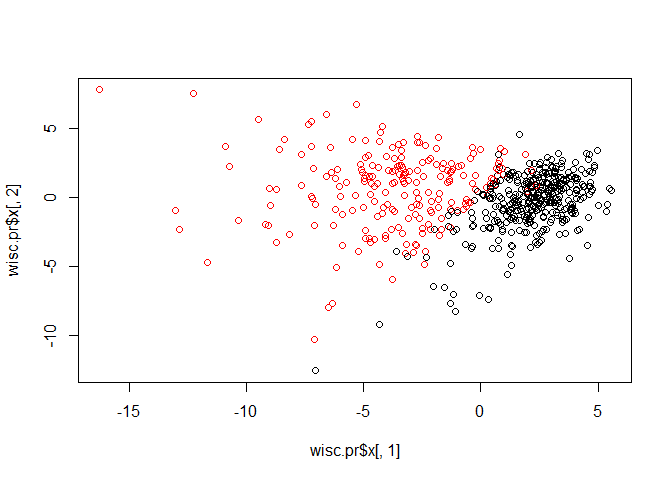
\includegraphics{CLASS_06_files/figure-latex/unnamed-chunk-23-1.pdf}

\begin{Shaded}
\begin{Highlighting}[]
\NormalTok{hc <-}\StringTok{ }\KeywordTok{hclust}\NormalTok{( }\KeywordTok{dist}\NormalTok{( }\KeywordTok{rbind}\NormalTok{(s1.b, s2.b, s3.b) ) )}
\KeywordTok{plot}\NormalTok{(hc)}
\end{Highlighting}
\end{Shaded}

\includegraphics{CLASS_06_files/figure-latex/unnamed-chunk-24-1.pdf}

\end{document}
